	\documentclass{clbeamer2024}

\usepackage{minted}

\usepackage{minted}
\setminted{
	breaklines=true,
	frame=single,
	bgcolor=lightgray,
	fontsize=\small,
	escapeinside=||
}

\usepackage{xcolor}
\definecolor{bg}{rgb}{0.95, 0.95, 0.92} % Couleur gris clair

\title{
	%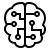
\includegraphics[width=0.5cm]{logos/IA1.png} \hfill
        Introduction aux Design Patterns
	
\includegraphics[width=0.7cm]{logos/data.png} \hfill
}
\subtitle{Comprendre les modèles de conception en programmation orientée objet}
\author{Slimani Mohamed Amine}
\institute{EHTP}
\date{\today}

\begin{document}
	\setcounter{framenumber}{-1}
	\frame{\titlepage}
	
	
	
	% Sommaire
	\begin{frame}{Sommaire}
		\tableofcontents
	\end{frame}
	
	
	\section{Qu'est-ce qu'un Design Pattern ?}
	\begin{frame}{Qu'est-ce qu'un Design Pattern ?}
		\begin{itemize}
			\item \textbf{Définition} : Un design pattern est une solution générique et réutilisable à un problème récurrent de conception logicielle.
			\item \textbf{Objectif} : Fournir une structure de code éprouvée pour résoudre des problèmes courants.
			\item \textbf{Avantages} : Réutilisabilité, maintenabilité, et meilleure communication entre développeurs.
		\end{itemize}
	\end{frame}
	
	
	\section{Pourquoi utiliser des Design Patterns ?}
	\begin{frame}{Pourquoi utiliser des Design Patterns ?}
		\begin{itemize}
			\item \textbf{Réutilisabilité} : Éviter de réinventer la roue pour des problèmes courants.
			\item \textbf{Maintenabilité} : Faciliter la compréhension et la modification du code.
			\item \textbf{Communication} : Utiliser un vocabulaire commun pour décrire des solutions.
		\end{itemize}
	\end{frame}
	
	
	\section{Catégories de Design Patterns}
	\begin{frame}{Catégories de Design Patterns}
		\begin{itemize}
			\item \textbf{Créationnels} : Concernent la création d'objets (ex. Singleton, Factory).
			\item \textbf{Structurels} : Concernent la composition d'objets (ex. Adapter, Decorator).
			\item \textbf{Comportementaux} : Concernent l'interaction entre objets (ex. Observer, Strategy).
		\end{itemize}
	\end{frame}
	
	
	\section{Exemples de Design Patterns}
	\begin{frame}{Exemples de Design Patterns}
		\begin{itemize}
			\item \textbf{Singleton} : Garantit qu'une classe n'a qu'une seule instance.
			\item \textbf{Factory} : Fournit une interface pour créer des objets.
			\item \textbf{Observer} : Permet à des objets de s'abonner à des événements.
		\end{itemize}
	\end{frame}
	
	
	\section{Exemple de code : Singleton}
	\begin{frame}{Exemple de code : Singleton}
		\begin{exampleblock}{Implémentation du Singleton en Java}
			
			\begin{center}
				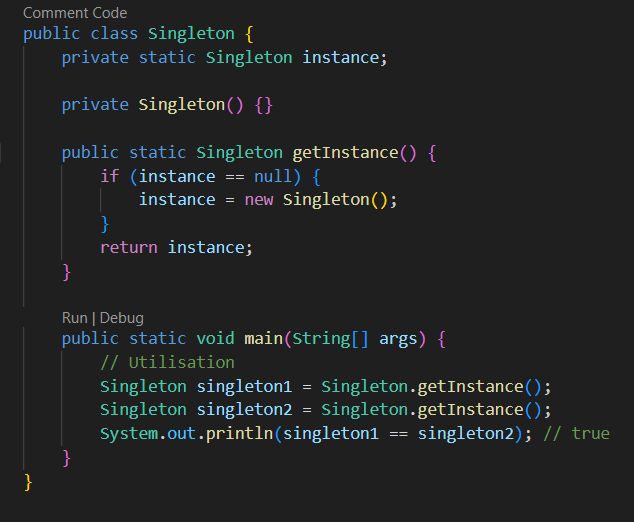
\includegraphics[width=0.7\textwidth]{images/code1.png}
			\end{center}
		
		\end{exampleblock}
	\end{frame}
	
	
	\section{Exemple de code : Factory}
	\begin{frame}{Exemple de code : Factory}
		\begin{exampleblock}{Implémentation du Factory en Java}
			\begin{center}
				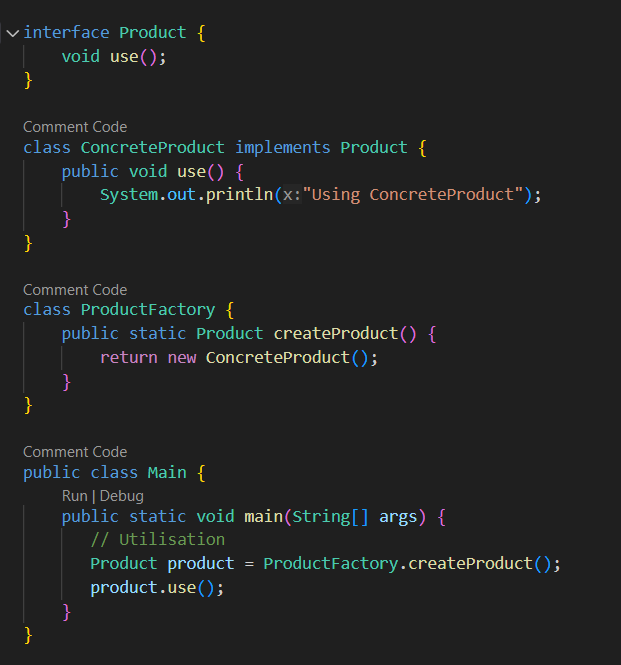
\includegraphics[width=0.63\textwidth]{images/code2.png}
			\end{center}
		\end{exampleblock}
	\end{frame}
	
	
	
	\section{Exemple de code : Observer}
	\begin{frame}{Exemple de code : Observer}
		\begin{exampleblock}{Implémentation de l'Observer en Java}
			
			\begin{center}
				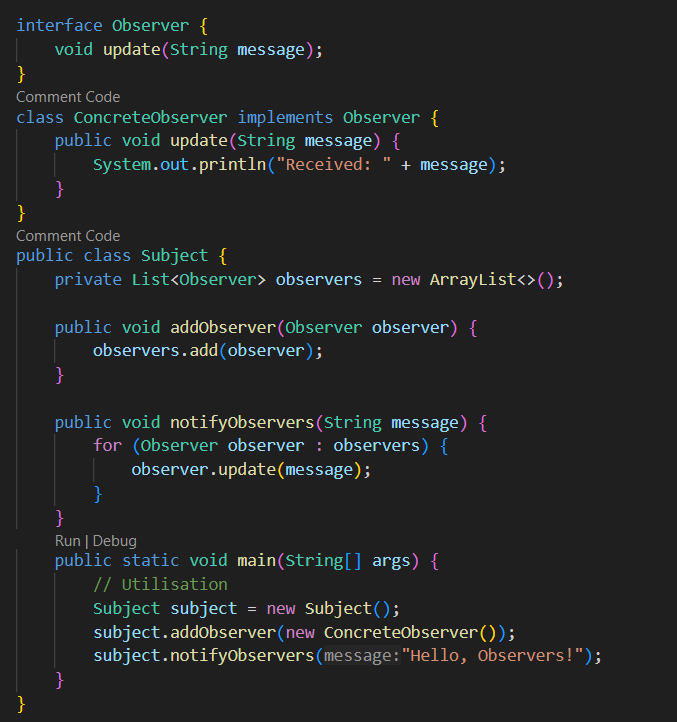
\includegraphics[width=0.63\textwidth]{images/code3.png}
			\end{center}
		
		\end{exampleblock}
	\end{frame}
	
	\section{Bonnes pratiques}
	\begin{frame}{Bonnes pratiques}
		\begin{itemize}
			\item \textbf{Choix du pattern} : Utiliser le bon pattern pour le bon problème.
			\item \textbf{Simplicité} : Ne pas surcharger le code avec des patterns inutiles.
			\item \textbf{Documentation} : Bien documenter l'utilisation des patterns.
		\end{itemize}
	\end{frame}
	
	
	\section{Outils pour travailler avec les Design Patterns}
	\begin{frame}{Outils pour travailler avec les Design Patterns}
		\begin{itemize}
			\item \textbf{UML} : Utiliser des diagrammes UML pour visualiser les patterns.
			\item \textbf{IDE} : Utiliser des IDE modernes pour faciliter l'implémentation.
			\item \textbf{Livres} : Se référer à des ouvrages comme "Design Patterns: Elements of Reusable Object-Oriented Software".
		\end{itemize}
	\end{frame}
	
	
	\section{Défis des Design Patterns}
	\begin{frame}{Défis des Design Patterns}
		\begin{itemize}
			\item \textbf{Complexité} : Certains patterns peuvent rendre le code plus complexe.
			\item \textbf{Surcharge} : Utiliser trop de patterns peut rendre le code difficile à comprendre.
			\item \textbf{Adaptation} : Adapter les patterns à des contextes spécifiques peut être difficile.
		\end{itemize}
	\end{frame}
	
	\section{Pourquoi c'est important ?}
	\begin{frame}{Pourquoi c'est important ?}
		\begin{itemize}
			\item Les design patterns sont essentiels pour écrire du code robuste et maintenable.
			\item Ils permettent de résoudre des problèmes courants de manière efficace.
			\item Comprendre les design patterns est crucial pour les développeurs expérimentés.
		\end{itemize}
	\end{frame}
	
	
	\begin{frame}{Résumé}
		\textbf{Les Design Patterns} sont des outils puissants pour améliorer la qualité du code.  
		Explorez, apprenez, et appliquez-les dans vos projets !
	\end{frame}
	
	
	

	
\end{document}
